\chapter{Common Noises in Guitar Recordings}

Noises can be separated into two categories, instrument and environment noises. We expect instrument and environment noises because in our use case, an online musical instrument course, we do not expect players to be experts, or to have access to an isolated recording environment. Our aim is to make an automatic assessment system robust to such noises. 

Most common instrument noises in amateur guitar recordings are \textit{slide} and \textit{buzz} noises. Slide noises are more common as they can be heard on all levels of performances. So common that they are artificially generated by guitar synthesizers to make the sound more realistic \cite{pakarinen2007analysis}. Buzz noises however, do occur most when the player is a beginner. Buzzing sound is considered unpleasant and unwanted. Another common noise is the percussive sound generated when right hand (or picking hand) touches excited strings. The touch could be intended to mute the string. The noise could also be intended, to add rhythmic percussion to the performance. In any case, it is classified as noise in this study. Environment noises are not predictable as instrument noises. There are too many possibilities for unwanted sounds in a non-ideal recording environment. One specific environment noise which might be expected in our use case is computer fan noise.

\section{Slide Noises}

Slide noises mostly happen during chord transitions. They occur when players move their hands while touching the strings. On nylon strings, they are much less audible. We focus on wound strings when we talk about slide noises. 

Pakarinen et al. \cite{pakarinen2007analysis} provides an analysis for these noise sounds. Sound consists two components. First, time-varying harmonics generated from interaction of finger and winding turns and second, static harmonics due to longitudinal vibration of the string. Energy of the time-varying harmonics are higher than static harmonics. 
\begin{equation}\label{slide_eq}
    f_H_n = nv_sd_w \quad, \quad n \in \mathbb{Z}^+
\end{equation}
Frequencies of the time-varying harmonics are linearly proportional to the speed of the finger (\(v_s\)) and wound density (\(d_w\)). As finger passes through each single winding turn, an impulse is created. Faster movement or denser winding turns result in shorter period between impulses. Static harmonics are due to vibration of the string, so they are not affected by the speed of the finger. Vibrations are only on longitudinal axis, since transversal vibrations are damped by the finger. Frequencies of the harmonics of longitudinal vibrations depend only on the length of the string and the density of its material. Therefore frequencies do not change with respect to location of sliding, but only their magnitudes.   
  
If the player tries to move his hand while still pressing on a string, the sliding noise will have higher initial energy and its pitch will be perceivable. In this form, the noise is often referred as a 'squeak' noise. The difference is the speed of the finger. Due to static friction between the string and the finger tip, the finger tip does not move immediately. While the player reduces the pressing force on the strings, at one moment, the force of static friction falls below the force acting on fingers parallel to the fret board, which was holding the whole arm from moving. Thus the instantaneous velocity of the finger at the moment it starts moving is much more higher than what it should be with a proper playing technique, causing an unpleasant 'squeak' sound. \\

Acceleration and deceleration of the hand between two frets causes frequencies of the time-varying harmonics to increase and then decrease (Figure \ref{fig:slide}). This trend was also found in \cite{pakarinen2007analysis}. 


\begin{figure}
    \centering
    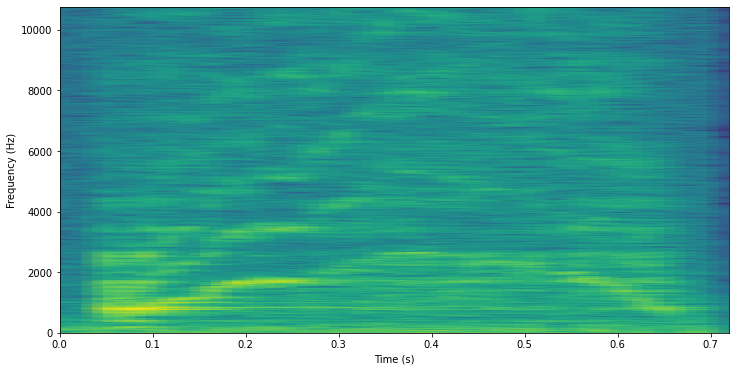
\includegraphics[width=\columnwidth]{methods/S_NR_A_12to3_stft.png}
    \caption{Short-time Fourier Transform magnitudes of the slide noise generated between 12th fret and 3rd fret of A string}
    \label{fig:slide}
\end{figure}

\section{Buzz Noises}\label{buzzsection}

These noises occur when a string collides with a fret during vibration. Collision of string and fret generates high frequency components. If the player does not apply enough pressing force between two frets, plucked string periodically leaves and collides with the fret of the note the player trying to play. Buzz noises also occur due to construction errors (e.g. unequal fret heights) or poor adjustments on the guitar (e.g. incorrect neck relief, height of the bridge and the nut).

Buzzing is a characteristic behaviour of Indian instrument sitar, and is not classified as a noise. Realistic synthesis of sitar sound requires modelling of the collision of strings and the bridge of the sitar. Vyasarayani et al. \cite{vyasarayani2009} models the movement of string in three phases. In first phase, plucked string do not contact with the obstacle (bridge). In second phase, the string partially wraps the obstacle. Lastly, the obstacle is completely wrapped. This description of string movement can be adapted to modelling of buzzing noise in the guitar. In case of guitar, obstacle is fret instead of bridge. One important difference is that the obstacle on guitar (fret) is circular and is never completely wrapped by the string. Third phase in movement of sitar string does not exist in guitar.     
  
Length of the string in motion is different in two phases (Figure \ref{fig:buzz}) . Length in first phase is greater than in second phase, by distance between the finger and the fret. If the buzzing is caused by weak force on the pressing finger (instead of an error on the guitar) we expect the frequency of produced sound to be lower due to the change of length. We see one example from our noise dataset on Figure \ref{fig:buzzstft}, where note B2 is played on E string (standard tuning). Buzz noise is generated by slowly releasing the string, which begins around 0.12 seconds. Fundamental frequency (F0) (Figure \ref{fig:buzzf0}) is obtained using YIN \cite{de2002yin} algorithm. F0 decreases from ~123 Hz (B2) towards ~116 Hz (A#2), but does not reach to it. Frequency of the decreased F0 depends on location of the finger on the fret.


\begin{figure}
    \centering
    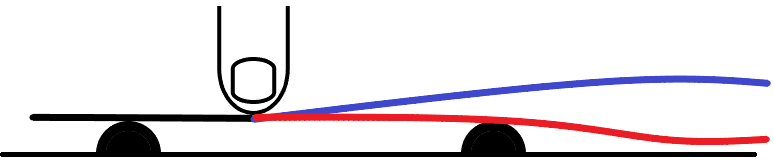
\includegraphics[width=\columnwidth]{methods/buzz_mov2.png}
    \caption{Phases of string motion during a buzz noise. Bottom line and half circles represent fretboard and frets. (Blue: Phase 1, Red: Phase 2)}
    \label{fig:buzz}
\end{figure}

\begin{figure}
    \centering
    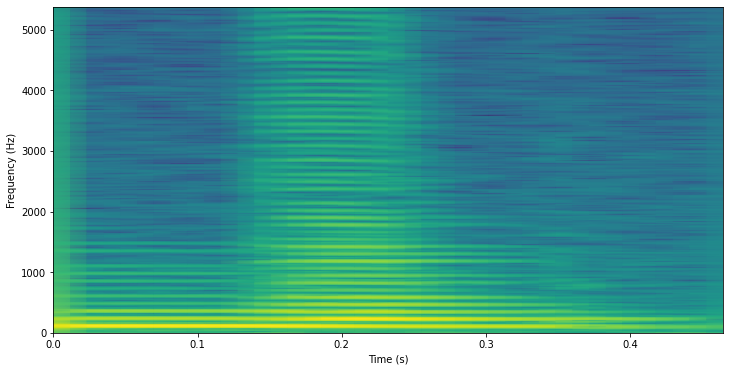
\includegraphics[width=\columnwidth]{methods/B_E_7_stft.png}
    \caption{Short-time Fourier Transform magnitudes of the buzz noise generated on 7th fret of E string}
    \label{fig:buzzstft}
\end{figure}

\begin{figure}
    \centering
    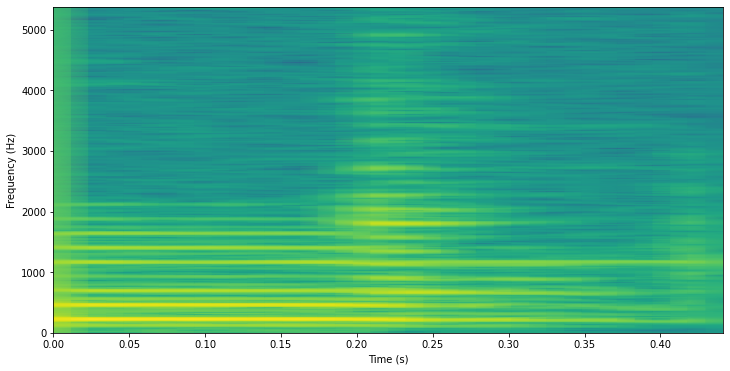
\includegraphics[width=\columnwidth]{methods/realbuzzstft.png}
    \caption{Short-time Fourier Transform magnitudes of the buzz noise in a recording from Music Critic dataset}
    \label{fig:realbuzz}
\end{figure}

\begin{figure}
    \centering
    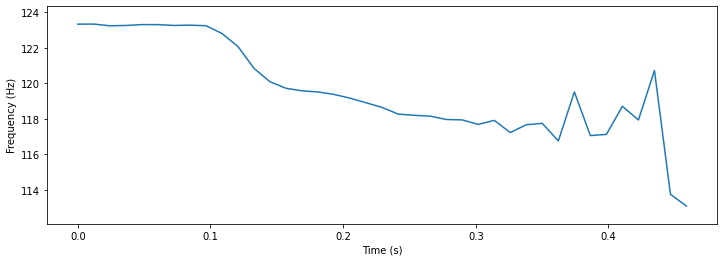
\includegraphics[width=\columnwidth]{methods/B_E_7_f0.png}
    \caption{Fundamental frequency of the buzz noise generated on 7th fret of E string}
    \label{fig:buzzf0}
\end{figure}

Buzz and slide noises cover most of the unintended noises in guitar recordings. There are also unpredictable noises that do not arise from fretboard and players hands, such as background noises or random sound producing events in the recording environment. Players may not have the complete control of their recording environment to prevent such noises. An onset detection algorithm must be robust to distinguish noises from players performance, just like a music teacher could do.